\documentclass[a4paper,14pt]{extarticle}

\usepackage{cmap}
\usepackage[T2A]{fontenc}
\usepackage[utf8x]{inputenc}
\usepackage[english, russian]{babel}

\usepackage{misccorr} % в заголовках появляется точка, но при ссылке на них ее нет
\usepackage{amssymb,amsfonts,amsmath,amsthm}  
\usepackage{indentfirst}
\usepackage[usenames,dvipsnames]{color} 
\usepackage[unicode,hidelinks]{hyperref}
% \hypersetup{%
%     pdfborder = {0 0 0}
% }
\usepackage{physics}

\usepackage{makecell,multirow} 
\usepackage{ulem}
\usepackage{graphicx,wrapfig}
\graphicspath{{img/}}
\usepackage{geometry}
\geometry{left=2cm,right=2cm,top=2cm,bottom=2cm,bindingoffset=0cm}
\usepackage{fancyhdr} 
\DeclareMathOperator{\Div}{div}
\DeclareMathOperator{\Rot}{rot}
\DeclareMathOperator{\Grad}{grad}
\DeclareMathOperator{\Const}{const}
\renewcommand{\phi}{\varphi}
\renewcommand{\epsilon}{\varepsilon}
\renewcommand{\kappa}{\varkappa}
\linespread{1.05} 
\frenchspacing 
\begin{document}
	\begin{center}
		\Large \textbf{Программа минимум по электродинамике}
	\end{center}
		\textit{Записать формулы и построить графики (без вывода), объяснить используемые в них обозначения: дать требуемые определения}
	\begin{enumerate}
		\item 
		\hyperlink{num1}{Запись функции, определяющей зависимость полей и векторных потенциалов гармонической плоской волны в линии передачи от времени $t$ и продольной координаты $z$. Понятия частоты, временного периода, продольного волнового числа, длины волны, фазовой и групповой скорости.}
		
		\item 
		\hyperlink{num2}{Волновое уравнение для векторного потенциала в отсутствие источников при произвольной и гармонической зависимости от времени. Дифференциальное уравнение для функций поперечных координат $\phi^{(e)}$ и $\phi^{(m)}$. Понятие поперечного волнового числа.}
		
		\item 
		\hyperlink{num3}{Понятие о TE, ТМ и ТЕМ волнах. Импедансная связь поперечных компонент полей. Определение поперечного волнового импеданса.}
		\item
		\hyperlink{num4}{Граничные условия для полей и функций  $\phi^{(e)}$ и $\phi^{(m)}$ в линиях передачи с идеально	
		проводящими границами. Математическая формулировка задачи отыскания собственных волн различных типов в идеальной линии.}
		\item 
		\hyperlink{num5}{Дисперсионное уравнение для волн в идеальных линиях. Понятие критической частоты и критической длины волны. Графики зависимости полей от продольной координаты в различные моменты времени при частотах, больших или меньших критической. Зависимости длины волны, фазовой и групповой скорости в линии передачи от частоты.}
		\item
		\hyperlink{num6}{В каких линиях могут существовать главные (TEM) волны? Поля TEM волны в коаксиальной линии.}
		\item 
		Спектр поперечных волновых чисел прямоугольного волновода. Низшая мода (поперечное волновое число, графики поля, картина силовых линий). Низшая мода круглого волновода (поперечное волновое число, картина силовых линий).
		\item
		Причины затухания волн в линиях передачи. Описание затухания, обусловленного потерями энергии в заполняющей среде. Графики зависимости поля в линии передачи с потерями от продольной координаты в различные моменты времени.
		\item 
		Описание главных волн в линиях передачи в терминах тока и напряжения: определения величин тока и напряжения, погонной емкости и индуктивности, \underline{определения} волнового сопротивления, импеданса нагрузки, импеданса в любом сечении линии с произвольной нагрузкой на конце.
		\item 
		Коэффициент отражения волны от нагрузки на конце линии. Понятие согласования линии с нагрузкой.
		\item 
		Спектр собственных частот идеального прямоугольного резонатора. Низшая мода прямоугольного резонатора (собственная частота, структура поля).
		\item 
		Причины затухания колебаний в реальных резонаторах. Описание затухания, обусловленного потерями энергии в заполняющей среде. График зависимости поля собственного колебания в реальном резонаторе от времени
		\item 
		Представление полей, создаваемых в волноводе заданными сторонними токами, в виде суперпозиции полей собственных мод (общий вид формул возбуждения волноводов)
		\item 
		Представление полей, создаваемых в резонаторе заданными сторонними токами, в виде суперпозиции полей собственных колебаний (общий вид формул возбуждения резонатора). Резонансные свойства полей.
		\item 
		Способы возбуждения волноводов и резонаторов при помощи штыря и петли.
		\item 
		Определения дифференциального и полного сечений рассеяния тела. Выражение для амплитуды поля и плотности потока энергии рассеянной волны в дальней зоне через дифференциальное сечение рассеяния.
		\item 
		Условие применимости приближения геометрической оптики в задачах дифракции.
		
	\end{enumerate}
	
	Задачи № 10.1 (а), 10.2, 10.4(а,б), 10.5(а,б), 10.7, 10.8, 10.16, 10.18(6), 10.19, 10.22, 10.23, 10.31(а,б), 10.33 (резонатор без плазмы), 10.35(a), 10.36, 10.38, 10.48, 11.1(1,2,3)
	(В.Б. Гильденбург, М.А. Миллер, Сборник задач по электродинамике, 2001 г.).
	\newpage
	\hypertarget{num1}{}
	Для плоской гармонической волны (TEM) функция, определяющая зависимость полей, задается следующим образом 
	
	$$\vec{A}^e = \phi^e(\vec{r}_\perp)e^{-ihz}\vec{z}_0$$
	
	Где $\vec{A}^e$ -- векторный потенциал поля, а $\phi^e(\vec{r}_\perp)$ называется поперечной волновой функцией. Поля $\vec{E}$ и $\vec{H}$ определяются следующим образом
	$$\vec{H}=\frac{1}{\mu} \Rot\vec{A}^e $$
	$$\vec{E}=-\frac{1}{c} \pdv{\vec{A}^e}{t}-\nabla{\phi} $$
	
	Где $\phi$ -- скалярный потенциал поля. 
	
	Используя условие калибровки Лоренца
	$$\Div\vec{A}^e+\frac{\epsilon\mu}{c}i\omega\phi=0$$
	
	Получим выражения для нахождения полей $\vec{E}$ и $\vec{H}$ в случае гармонической волны:
	$$\vec{H}=\frac{1}{\mu} \Rot\vec{A}^e $$
	$$\vec{E}=\frac{1}{i k_0\epsilon\mu}(\nabla \Div + k^2)\vec{A}^e $$
	$$k_0=\frac{\omega}{c}, \quad k=\frac{\omega}{c}\sqrt{\epsilon\mu}$$
	
	Понятие частоты $\omega$ -- равна количеству повторений или возникновения событий (процессов) в единицу времени.
	
	Понятие временного периода $T = \frac{2\pi}{\omega}$ -- время, за которое совершается полное колебание.
	
	Понятие продольного волнового числа $h=\frac{2\pi}{\lambda}$ -- волновым числом  называется быстрота роста фазы волны по пространственной продольной координате.
	
	Понятие длины волны $\lambda$ -- пространственный период колебаний. Расстояние между двумя ближайшими друг к другу точками в пространстве, в которых колебания происходят в одинаковой фазе.
	
	Понятие фазовой $v_{\text{ф}}$ и групповой скорости $v_{\text{гр}}$. Фазовая скорость -- скорость перемещения поверхности постоянной фазы. Групповая скорость -- скорость перемещения квазимонохроматического пакета.
	$$v_{\text{ф}}=\frac{\omega}{h}, \quad v_{\text{гр}}=\pdv{\omega}{h} \Bigl|_{\omega=\omega_0}$$
	Где $\omega_0$ -- несущая частота группового пакета.
	
	\newpage
	\hypertarget{num2}{}
	Волновое уравнение для векторного потенциала в случае произвольной зависимости от времени и отсутствия сторонних источников
	$$\Delta\vec{A} -\frac{\epsilon\mu}{c^2}\pdv[2]{\vec{A}}{t}=0$$ 
	
	Волновое уравнение для векторного потенциала в случае гармонической зависимости от времени и отсутствия сторонних источников
	$$\Delta\vec{A} + k^2 \vec{A}=0$$
	$$\pdv{}{t} \to i\omega, \quad k^2=\frac{\omega^2}{c^2}\epsilon\mu$$
	
	Дифференциальное уравнение для функций поперечных координат $\phi^{(e)}$ и $\phi^{(m)}$. Понятие поперечного волнового числа.
	$$\vec{A}^e = \phi^e(\vec{r}_\perp)e^{-ihz}\vec{z}_0$$
	$$\Delta = \pdv[2]{}{x}+\pdv[2]{}{y}+\pdv[2]{}{z}=\Delta_\perp+\pdv[2]{}{z}$$ -- для декартовой системы координат.
	$$\Delta A_z^e + k^2 A_z^e=\Delta_\perp\phi^e + (k^2-h^2)\phi^e=0$$
	Тогда дифференциальное уравнение для функций поперечных координат $\phi^{(e)}$ и $\phi^{(m)}$  выглядит следующим образом
	$$\Delta_\perp\phi^{(e,m)} + \kappa^2\phi^{(e,m)}=0$$
	Где $\kappa$ -- поперечное волновое число. 	
	
	Если функции $\phi^{(e)}$ и $\phi^{(m)}$ удовлетворяют двумерному уравнению Гельмгольца, то поля удовлетворяют уравнению Максвелла.
	
	\newpage
	\hypertarget{num3}{}
	Используем выражения для полей через векторный потенциал
	$$\vec{H}=\frac{1}{\mu} \Rot\vec{A}^e $$
	$$\vec{E}=\frac{1}{k_0\epsilon\mu}(\nabla \Div + k^2)\vec{A}^e $$
	
	Вычислим $\nabla div \vec{A}^e$ и $rot \vec{A}^e$ при условии $\vec{A}^e = \phi^e(\vec{r}_\perp)e^{-ihz}\vec{z}_0$
	$$\Div \vec{A}^e = -ih\phi^e(\vec{r}_\perp)e^{-ihz}$$
	$$\nabla \Div \vec{A}^e = (-h^2\phi^e\vec{z}_0-ih\nabla_\perp\phi^e)e^{-ihz}$$
	$$\Rot \vec{A}^e = [\nabla A^e_z,\vec{z}_0] = [\nabla_\perp\phi^e,\vec{z}_0]e^{-ihz}$$
	
	Тогда получим следующие выражения для комплексных амплитуд полей TM волны 
	\begin{displaymath}
	e^{-ihz}\cdot
	\begin{cases}
	$$\displaystyle E_z = \frac{\kappa^2}{k_0\epsilon\mu}\phi^e(\vec{r}_\perp)$$ \\
	$$\displaystyle\vec{E}_\perp = -\frac{h}{k_0\epsilon\mu}\nabla_\perp\phi^e(\vec{r}_\perp)$$ \\
	$$\displaystyle\vec{H}_\perp = \frac{1}{\mu}[\nabla_\perp\phi^e(\vec{r}_\perp,\vec{z}_0)]$$ \\
	$$\displaystyle H_z = 0$$
	\end{cases}
	\end{displaymath}

	TM - поперечная магнитная волна. Магнитное поле чисто поперечно пути распространения, но поле $\vec{E}=\vec{E}_\parallel+\vec{E}_\perp$ имеет продольную и поперечную составляющую.
	
	Уравнения Максвелла симметричны относительно полей, но мы получили неравноправные выражения для векторов. Это объясняется тем, что мы нашли одно из решений. Воспользовавшись принципом двойственности $\vec{E}\to\vec{H}$, $\vec{H}\to -\vec{E}$, можно получить выражения  для комплексных амплитуд полей TE волны. 
	\begin{displaymath}
	e^{-ihz}\cdot
	\begin{cases}
	$$\displaystyle H_z = \frac{\kappa^2}{k_0\epsilon\mu}\phi^e(\vec{r}_\perp)$$ \\
	$$\displaystyle\vec{H}_\perp = -\frac{h}{k_0\epsilon\mu}\nabla_\perp\phi^e(\vec{r}_\perp)$$ \\
	$$\displaystyle\vec{E}_\perp = -\frac{1}{\epsilon}[\nabla_\perp\phi^e(\vec{r}_\perp,\vec{z}_0)]$$ \\
	$$\displaystyle E_z = 0$$
	\end{cases}
	\end{displaymath}
	
	функция $\phi$ не обязана быть такой же, поэтому изменяется верхний индекс на $m$, эта функция также должна удовлетворять уравнению Гельмгольца  
	$$\Delta_\perp\phi^{m} + \kappa^2\phi^{m}=0$$
	
	Таким образом для системы уравнений Максвелла возможны два решения TM и TE волны. Но есть случай, когда поля чисто поперечны это случай TEM волны.
	Когда $\kappa = 0$, то есть $k=h$, продольные компоненты магнитного и электрического полей отсутствуют это и есть TEM волна.
	\begin{displaymath}
	e^{-ihz}\cdot
	\begin{cases}
	$$\displaystyle H_z = E_z = 0$$ \\
	$$\displaystyle\vec{E}_\perp = -\frac{1}{\epsilon\mu}\nabla_\perp\phi(\vec{r}_\perp)$$ \\
	$$\displaystyle\vec{H}_\perp = \frac{1}{\mu}[\nabla_\perp\phi(\vec{r}_\perp,\vec{z}_0)]$$ 
	\end{cases}
	\end{displaymath}
	
	$\phi$ -- поперечная волновая функция, удовлетворяющая уравнению $\Delta\phi=0$.
	
	Из формул выше видно, что поперечные компоненты полей удовлетворяют импедансному соотношению
	$$\vec{E}_\perp = \eta_{\perp\text{в}}[\vec{H}_\perp,\vec{z}_0]$$
	
	где $\eta_{\perp\text{в}}$ называется поперечным волновым сопротивлением
	$$\eta_{\perp\text{в}}=\sqrt{\frac{\mu}{\epsilon}} \left( \frac{k}{h} \right)^{\pm 1}$$ 
	
	<<+>> -- соответствует волне типа TE, а <<-->> -- волне типа TM. Для TEM волны $\displaystyle \eta_{\perp\text{в}}=\sqrt{\frac{\mu}{\epsilon}}$
	
	\newpage
	\hypertarget{num4}{}
	\begin{figure}[h!]
		\centering
		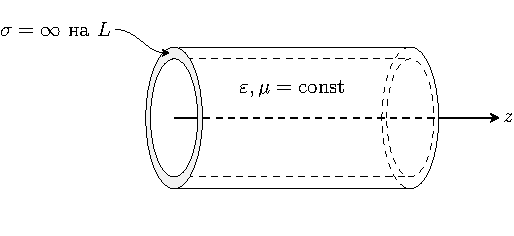
\includegraphics[scale=1.5]{img/lect2_ris1}
		\caption{Линия передачи}
		\label{fig:wavegain:1}
	\end{figure}
	Поперечные волновые функции удовлетворяют двумерному уравнению Гельмгольца
	$$\Delta_\perp\phi^{(e,m)}+\kappa^2\phi^{(e,m)}=0$$
	
	На границе проводящих стенок справедливы следующие граничные условия
	$$E_\tau = 0 |_S, \quad B_n = 0 |_S$$
	
	Рассмотрим граничные условия для функций $\phi^{(e,m)}$ для различных типов волн.
	
%	TM-волна. $\phi^e$
%	
%	$E_z=0, \quad, E_{\perp\tau}=0$ на границе.
%	
%	$E_z\sim \phi^e(\vec{r}\perp) \Rightarrow \phi^e|_S = 0$
%	
%	Граничное условие для TM волны.
%	\vspace{20pt}
%	
%	TE-волна. $\phi^m$
%	
%	$E_{\perp\tau}=0$ на границе.
%	
%	$\displaystyle E_{\perp\tau}\sim ([\nabla\phi^m(\vec{r}\perp),\vec{z}_0],\vec{\tau}) \Rightarrow \pdv{\phi^e}{n}\Bigl|_S = 0$
%
%	Граничное условие для TE волны.
%	\vspace{20pt}
%	
%	TEM-волна. $\phi$
%	
%	$\vec{E}_{\perp}\sim \nabla\phi$
%	
%	$\displaystyle \pdv{\phi}{n}\Bigl|_S = 0 \Rightarrow \phi|_S=\Const$
%	
%	Граничное условие для TEM волны.
%	
%	Важно, что эта $\Const$ может быть разной на разных проводниках (пример коаксиальная линия).
%	\newpage
	Математическая формулировка задачи описания волн в линии передач.
	
	TM
	
	$\Delta_\perp\phi^{e}+\kappa^2\phi^{e}=0$
	
	$\phi^e|_L = 0$
	Условие Дирихле.
	\vspace{20pt}
	
	TE
	
	$\Delta_\perp\phi^{m}+\kappa^2\phi^{m}=0$
	
	$\displaystyle \pdv{\phi^m}{n}|_L = 0$
	Условие Неймана.
	
	Где $\vec{n}$ -- нормаль к контуру $L$ на границе поперечного сечения.
	\vspace{20pt}
	
	TEM
	
	$\Delta_\perp\phi=0$
	
	$\phi|_{L_i} = C_i$
	
	Таким образом описание волн в линии передач сводится к двумерной задачи Гельмгольца с следующими граничными условиями на контуре, охватывающим поперечное сечение волновода.
	
	\newpage
	\hypertarget{num5}{}
	Дисперсионное соотношение 
	$$\kappa^2 = k^2 - h^2 = \frac{\omega^2}{c^2}\epsilon\mu - h^2$$
	\begin{figure}[h!]
		\centering
		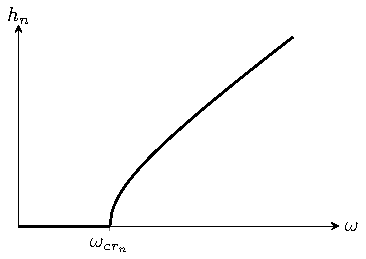
\includegraphics[scale=1.6]{img/lect2_ris6}
		\caption{Зависимость реальной части поперечного волнового числа от частоты}
		\label{fig:wavegain:5}
	\end{figure}
	Где $\kappa$ -- поперечное волновое число, а $h$ - продольное волновое число. 
	
Любая мода в линии передачи характеризуется поперечным волновым числом, а поперечное волновое число определяет продольное.

Можем ввести критическую длину волны (продольное волновое число $h$ равно нулю):
\begin{gather*}
\kappa^2 = {\frac{\omega}{c}}^2 {\epsilon \mu}\\
\omega_{cr} = \frac{\kappa c}{\sqrt{\epsilon \mu}}\\
\lambda = \frac{2 \pi c}{\omega_{cr}} = \frac{2 \pi}{\kappa \sqrt{\epsilon \mu}}
\end{gather*}
$\omega < \omega_{cr}$ дисперсионное уравнения не имеет действительных решений -- режим нераспространяющейся волны. 

При  $\omega > \omega_{cr}$ -- режим распространяющейся волны.

%Если волна бежит вправо, то $h > 0$; если бежит влево, то $h < 0$
%
%\begin{equation*}
%Re{\vec{E}} , Re{\vec{H}} \sim \cos(\omega t - h z)
%\end{equation*}

\begin{figure}[h!]
	\centering
	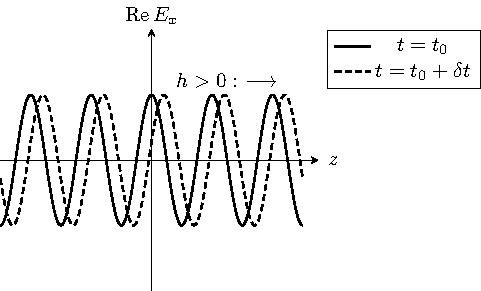
\includegraphics[scale=1]{img/lect3_ris1}
	\caption{Распространение волны ($h>0$)}
	\label{fig:lect3:1}
\end{figure}
%При $\omega < \omega_{cr}$
%\begin{equation*}
%h = \pm i |h|
%\end{equation*}

%\begin{equation*}
%Re{E_x} \sim \cos(\omega t + \phi_0) \exp{\mp |h| z}
%\end{equation*}

Бегучести нет.
Зависимость экспоненциальная
\begin{figure}[h!]
	\centering
	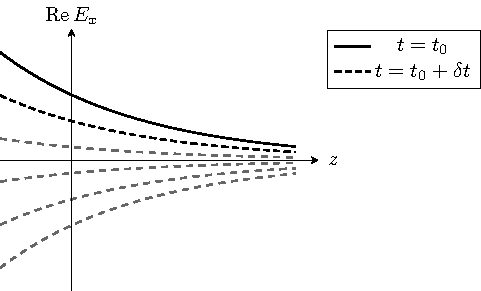
\includegraphics[scale=1]{img/lect3_ris2}
	\caption{Режим нераспространения ($h<0$)}
	\label{fig:lect3:2}
\end{figure}

\begin{figure}[h!]
	\centering
	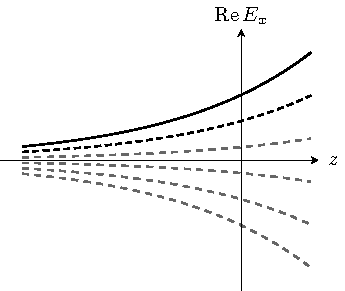
\includegraphics[scale=1]{img/lect3_ris3}
	\caption{Экспоненциальное нарастание амплитуды (при $h<0$)}
	\label{fig:lect3:3}
\end{figure}
%Картинка зависит от способа создания волны, то есть у экспоненты << +>> или <<-->>. В зависимости от того, где источник можем сказать, куда бежит волна. То есть определить знак.
%
%Источник может порождать несколько мод, но не все, а какие-то конкретные.
%\begin{figure}[h!]
%	\centering
%	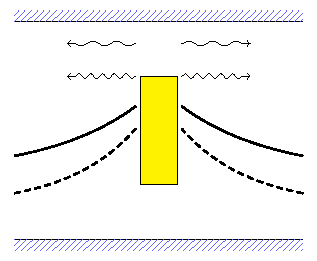
\includegraphics[scale=1]{img/lect3_ris4}
%	\caption{Моды в линии передачи с источником}
%	\label{fig:lect3:4}
%\end{figure}
%Изобразим числовую ось.
%Пусть задана $\omega$, а то есть $k = \frac{\omega}{c} \sqrt{\epsilon \mu}$
%
%Если $k < \kappa_1$ - все моды нераспространяющиеся.
%
%Когда $k$ перейдёт через $\kappa_1$ появится низшая мода.
%
%Когда перейдём через $\kappa_2$  появится ещё одна критическая частота.
%
%!!Можно дополнить описание числовой прямой!!
%\begin{figure}[h!]
%	\centering
%	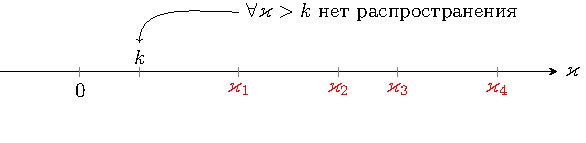
\includegraphics[scale=1]{img/lect3_ris5}
%	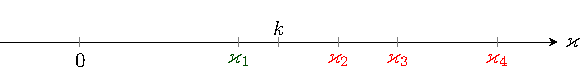
\includegraphics[scale=1]{img/lect3_ris6}
%	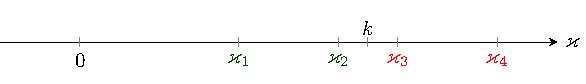
\includegraphics[scale=1]{img/lect3_ris7}
%	% \label{fig:lect3:4}
%\end{figure}
%
%Кинематические соотношения
%
%Определяют кинематические параметры волны.
%
\begin{enumerate}
%	\item Временной период 
%	
%	\begin{equation*}
%	T = \frac{2 \pi}{\omega}
%	\end{equation*}
	
	\item Длина волны в волноводе (подразумевают линию передачи или трубу, когда говорят волновод)
	\begin{equation*}
	\lambda_v = \frac{2 \pi}{h} = \frac{2 \pi}{\sqrt{k^2 - \kappa^2}} = \frac{2 \pi}{k} \frac{1}{\sqrt{1 - \frac{\kappa^2}{k^2}}} = \frac{\lambda_0}{\sqrt{1 - \frac{\omega_cr^2}{\omega}}} > \lambda_0
	\end{equation*}
	
	Когда $\omega \rightarrow \omega_{cr}$	$\lambda_{v} \rightarrow \infty$
	
	$\lambda_0$ - длина волны в пространстве без волновoда в той же среде.
	
	$\lambda_{v}$ - пространственный период.
	
	\item Фазовая скорость - скорость перемещения плоскости постоянной фазы.
	
	Поверхность постоянной фазы - это когда фаза константа.
	\begin{equation*}
	faza = \omega t - h z + \phi_0
	\end{equation*}
	
	При данном времени можно найти координату:
	\begin{equation*}
	z = \frac{\omega t  + \phi_0}{ h }
	\end{equation*}
	
	Координата будет перемещаться со скоростью:
	\begin{equation*}
	v_f = \frac{\omega}{h}
	\end{equation*}
	\begin{equation*}
	v_f = 
	\frac{\omega}{\sqrt{k^2 - \kappa^2}} = 
	\frac{\omega}{k} \frac{1}{\sqrt{1 - {\frac{k}{\kappa}^2}}} = \frac{\omega}{k} \frac{1}{\sqrt{1 - {\frac{\omega_{cr}}{\omega}^2}}} > v_f^{(0)}
	\end{equation*}
	\begin{equation*}
	v_f^{(0)} = \frac{c}{\varepsilon \mu} = \frac{\omega}{k}
	\end{equation*}
	Фазовая скорость может быть больше скорости света.
	
	\item Групповая скорость - скорость перемещения квазимонохроматического волнового пакета. 	
%	\begin{figure}[h!]
%		\centering
%		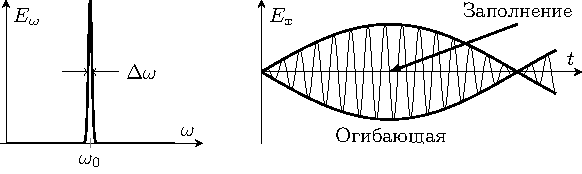
\includegraphics[scale=1]{img/lect3_ris8}
%		\caption{Квазимонохроматический волновой пакет}
%		\label{fig:lect3:8}
%	\end{figure}
	
%	Сигнал характеризуется высокочастотным заполнением и огибающей.
	
%	\begin{figure}[h!]
%		\centering
%		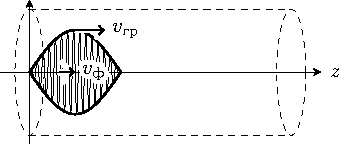
\includegraphics[scale=1]{img/lect3_ris9}
%		\caption{Распространение волнового пакета}
%		\label{fig:lect3:9}
%	\end{figure}
%	По сути это радиоимпульс.
	
	Пакет движется со скоростью $ v_{gr} = \pdv{\omega}{k}\vert_{\omega = \omega_{0}} $ -- это при малом или отсутствующем поглощении.(В пространстве, а не в линии передачи).
	
	При большом поглощении это понятие теряет смысл.
	
	По мере перемещения по волноводу форма сигнала будет меняться.
	
	$v_{gr} = \pdv{\omega}{h}\vert_{\omega = \omega_{0}} $ - формула для волновода. 
	
%	\begin{gather}
%	k^2 = h^2 + \kappa^2\\
%	%
%	k = \frac{\omega}{c} \sqrt{ \varepsilon \mu}
%	\end{gather}
%	
%	Берём дифференциал от правой и левой части.$\kappa$  не зависит от частоты.
%	\begin{gather*}
%	2k dk = 2h dh\\
%	\pdv{\omega}{h} = \frac{c}{\sqrt{\varepsilon \mu}} \frac{h}{k}\\
%	h = + \sqrt{\frac{\omega^2}{c^2} \varepsilon \mu -\kappa^2_n}\\
%	\pdv{\omega}{h} = \frac{c}{\sqrt{\varepsilon \mu}} \frac{c}{\omega \sqrt{\varepsilon \mu}} \sqrt{\frac{\omega^2}{c^2} \varepsilon \mu -\kappa^2_n} = \frac{{v_f^{(0)}}^2}{v_f}
%	\end{gather*}
%	
%	\begin{gather*}
%	v_{f} = \frac{\omega}{h}\\
%	v_{f}^{(0)} = \frac{c}{\omega \sqrt{\varepsilon \mu}}\\
%	%
%	v_{f} v_{gr} = {v_f^{(0)}}^2
%	\end{gather*}
%	\begin{equation*}
%	v_{gr} = v_{f}^{(0)} \sqrt{1 - {\frac{\omega_{cr}}{\omega}^2}}
%	\end{equation*}
%	
%	Всё это справедливо для сред без временной дисперсии.
%	\begin{equation*}
%	\varepsilon\ne f(\omega), \mu \ne f(\omega)
%	\end{equation*}
%	
%
%	
%	$v_{gr} < c$ - она несёт информацию.
\end{enumerate}
%\begin{figure}[h!]
%	\centering
%	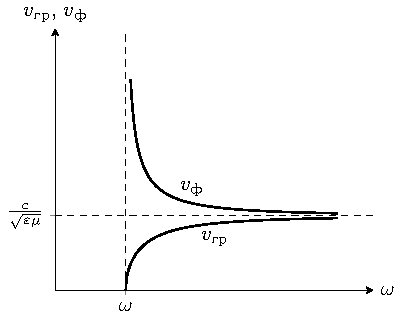
\includegraphics[scale=1]{img/lect3_ris10}
%	\caption{Распространение волнового пакета}
%	\label{fig:lect3:10}
%\end{figure}

\newpage
\hypertarget{num6}{}
Главные (TEM) волны в линиях передачи с идеальными границами

У TEM-волн поперечное волновое число $\varkappa=0$:
\begin{equation*}
\varkappa=0 \Rightarrow h=k= \frac{\omega}{c}\sqrt{\varepsilon \mu}
\end{equation*}
Поля таких волн выражаются следующим образом через функцию $\varphi$:
\begin{gather*}
\label{eperp}
\vec{E}_\perp=-\frac{1}{\sqrt{\varepsilon \mu}}\nabla_\perp \varphi\\
\vec{H}_\perp=-\frac{1}{\mu}\qty[\nabla_\perp \varphi,\vec{z}_0]
\end{gather*}

%При этом выполняются \textbf{граничные условия}: на каждом из проводников (допустим, есть набор проводников, вдоль которых распространяется волна)
%\begin{equation*}
%\varphi|_{l_i}=C_i,
%\end{equation*}
%причем константа не обязана быть одна для всех проводников.
%
%\begin{figure}[h!]
%	\centering
%	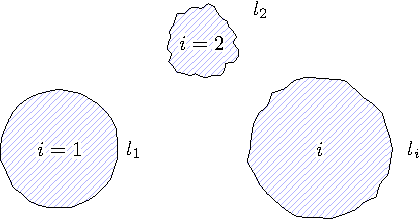
\includegraphics[scale=1]{img/lect4_ris1}
%	\caption{Набор проводников в задаче}
%	\label{fig:lect4:1}
%\end{figure}
%
%\textbf{Внутренняя задача}
%
%\begin{figure}[h!]
%	\centering
%	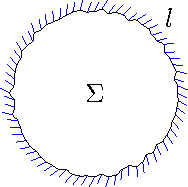
\includegraphics[scale=1]{img/lect4_ris2}
%	\caption{Случай одного проводника}
%	\label{fig:lect4:2}
%\end{figure}
%Пусть у нас есть только один проводник, в котором есть цилиндрическая полость (рис. \ref{fig:lect4:2}). Рассмотрим внутреннюю задачу, т.е. распространение волны внутри цилиндрической полости. Оказывается, для граничного условия $\varphi_\perp|_l=C_1$ существует только тривиальное решение $\varphi_\perp=C_1$. Для доказательства необходимо воспользоваться теоремой и минимуме и максимуме для гармонической функции.
%%\begin{equation*}
%%\Delta \varphi=\Div\qty(\varphi\nabla \varphi)=0 \quad \bigg| \iint\limits_\Sigma
%%\end{equation*}
%%Это такая задача, которую проще доказать самому. Попробуйте это сделать сами.
%
%\textbf{Внешняя задача}
%
%Зададимся вопросом о решении той же задачи:
%\begin{equation*}
%\Delta_\perp \varphi=0, \quad \varphi|_l=\mathrm{const}
%\end{equation*}
%Только теперь будем рассматривать её в области вне проводника
%
%Для начала рассмотрим задачу попроще, поле нити (рис. \ref{fig:lect4:3}). Её решение известно:
%\begin{equation*}
%\Delta_\perp \varphi=0 
%\quad \Rightarrow \quad
%\varphi \sim \ln r
%\end{equation*} 
%
%Характер убывания полей здесь $\displaystyle E_r\sim \frac{1}{r}$, а для магнитного поля в силу импедансного соотношения $\displaystyle\frac{E_r}{H_\phi}=\eta_{\perp\text{в}}=1, \quad H_\varphi\sim\frac{1}{r}$:
%\begin{equation*}
%E_r=H_\phi\sim\frac{1}{r}
%\end{equation*}
%\begin{figure}[h!]
%	\centering
%	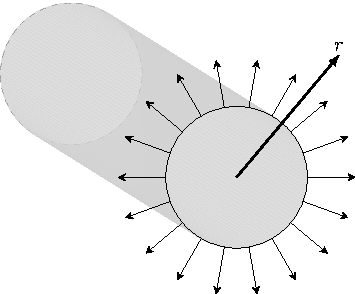
\includegraphics[scale=1.5]{img/lect4_ris3}
%	\caption{Поле бесконечной проводящей нити}
%	\label{fig:lect4:3}
%\end{figure}
%
%Посмотрим на поведение полей при $r\to\infty$. Говорят, нужно поставить граничные условия (или закон убывания) на бесконечности. Чем плох закон $\frac{1}{r}$?
%
%Посчитаем средний по времени поток энергии через поперечное сечение, в котором распространяется волна. Сечение бесконечно, за исключением конечной площади проводника.
%
%Сначала вычислим вектор Пойнтинга (средний по времени и в проекции на $z$):
%\begin{equation*}
%\overline{S}_z=\frac{c}{8 \pi}\mathrm{Re}\qty(E_r\cdot H_\phi^*)\sim\frac{1}{r^2}
%\end{equation*}
%\begin{equation*}
%\Pi=\iint\limits_\Sigma \overline{S}_z ds \sim
%\iint\limits_\Sigma \frac{1}{r^2} (2\pi r \dd{r})
%\sim \int\limits_a^\infty = \ln\frac{\infty}{a}=\infty
%\end{equation*}
%Интеграл расходится на бесконечности. Говорят, что расходимость носит логарифмический характер. Получили бесконечную мощность волны: такую волну невозможно создать реальным источником --- волна не удовлетворяет критерию энергетической реализуемости.

\textbf{вдоль одиночного проводника TEM-волна с конечной энергией распространятся не может}. Распространение возможно, если количество проводников будет больше одного. Например, в линии из двух проводников (рис. \ref{fig:lect4:4}) TEM-волна уже возможна.

\begin{figure}[h!]
	\centering
	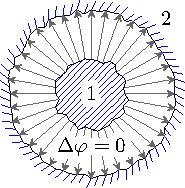
\includegraphics[scale=1.5]{img/lect4_ris4}
	\caption{Закрытая линия из двух проводников}
	\label{fig:lect4:4}
\end{figure}

%Можно модифицировать задачу с нитью (рис. \ref{fig:lect4:5}):
%
%\begin{figure}[h!]
%	\centering
%	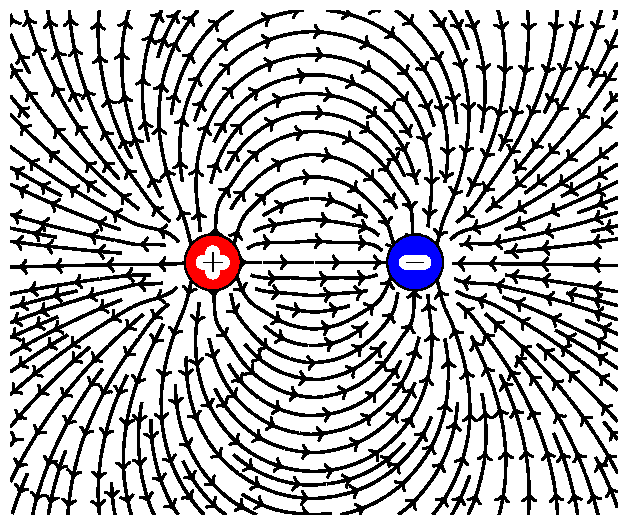
\includegraphics[scale=0.7]{img/lect4_ris5}
%	\caption{Поле двухпроводной линии}
%	\label{fig:lect4:5}
%\end{figure}
%
%В поперечном разрезе это поле диполя, а оно спадает быстрее, $\sim \frac{1}{r^2}$. Тогда
%\begin{equation*}
%E_\perp\sim H_\perp \sim \frac{1}{r^2}
%\quad \Rightarrow \quad
%\overline{S}_z \sim \frac{1}{r^4}, \quad
%\Pi \sim \int\limits_{L_\text{характ}}^\infty \frac{1}{r^3} \dd{r}
%\end{equation*}
%
%Мощность волны конечна, значит, в модифицированной задаче TEM-волна энергетически реализуема.

 TEM-волна в идеальной линии передачи возможна, если число проводников $\geq 2$.

Например, в коаксиальной линии (рис. \ref{fig:lect4:6}) TEM-волна возможна.

\begin{figure}[h!]
	\centering
	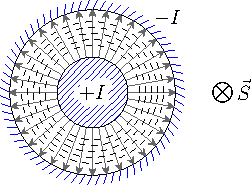
\includegraphics[scale=1.5]{img/lect4_ris6}
	\caption{Поле в коаксиальном кабеле}
	\label{fig:lect4:6}
\end{figure}

%Зададимся вопросом: возможны ли в такой линии TE и TM волны? Сформулируем утверждение, пока без доказательства: \textbf{в открытых линиях передачи TE и TM волны не существуют}.
\end{document}